% Options for packages loaded elsewhere
\PassOptionsToPackage{unicode}{hyperref}
\PassOptionsToPackage{hyphens}{url}
\documentclass[
]{article}
\usepackage{xcolor}
\usepackage[margin=1in]{geometry}
\usepackage{amsmath,amssymb}
\setcounter{secnumdepth}{-\maxdimen} % remove section numbering
\usepackage{iftex}
\ifPDFTeX
  \usepackage[T1]{fontenc}
  \usepackage[utf8]{inputenc}
  \usepackage{textcomp} % provide euro and other symbols
\else % if luatex or xetex
  \usepackage{unicode-math} % this also loads fontspec
  \defaultfontfeatures{Scale=MatchLowercase}
  \defaultfontfeatures[\rmfamily]{Ligatures=TeX,Scale=1}
\fi
\usepackage{lmodern}
\ifPDFTeX\else
  % xetex/luatex font selection
\fi
% Use upquote if available, for straight quotes in verbatim environments
\IfFileExists{upquote.sty}{\usepackage{upquote}}{}
\IfFileExists{microtype.sty}{% use microtype if available
  \usepackage[]{microtype}
  \UseMicrotypeSet[protrusion]{basicmath} % disable protrusion for tt fonts
}{}
\makeatletter
\@ifundefined{KOMAClassName}{% if non-KOMA class
  \IfFileExists{parskip.sty}{%
    \usepackage{parskip}
  }{% else
    \setlength{\parindent}{0pt}
    \setlength{\parskip}{6pt plus 2pt minus 1pt}}
}{% if KOMA class
  \KOMAoptions{parskip=half}}
\makeatother
\usepackage{color}
\usepackage{fancyvrb}
\newcommand{\VerbBar}{|}
\newcommand{\VERB}{\Verb[commandchars=\\\{\}]}
\DefineVerbatimEnvironment{Highlighting}{Verbatim}{commandchars=\\\{\}}
% Add ',fontsize=\small' for more characters per line
\usepackage{framed}
\definecolor{shadecolor}{RGB}{248,248,248}
\newenvironment{Shaded}{\begin{snugshade}}{\end{snugshade}}
\newcommand{\AlertTok}[1]{\textcolor[rgb]{0.94,0.16,0.16}{#1}}
\newcommand{\AnnotationTok}[1]{\textcolor[rgb]{0.56,0.35,0.01}{\textbf{\textit{#1}}}}
\newcommand{\AttributeTok}[1]{\textcolor[rgb]{0.13,0.29,0.53}{#1}}
\newcommand{\BaseNTok}[1]{\textcolor[rgb]{0.00,0.00,0.81}{#1}}
\newcommand{\BuiltInTok}[1]{#1}
\newcommand{\CharTok}[1]{\textcolor[rgb]{0.31,0.60,0.02}{#1}}
\newcommand{\CommentTok}[1]{\textcolor[rgb]{0.56,0.35,0.01}{\textit{#1}}}
\newcommand{\CommentVarTok}[1]{\textcolor[rgb]{0.56,0.35,0.01}{\textbf{\textit{#1}}}}
\newcommand{\ConstantTok}[1]{\textcolor[rgb]{0.56,0.35,0.01}{#1}}
\newcommand{\ControlFlowTok}[1]{\textcolor[rgb]{0.13,0.29,0.53}{\textbf{#1}}}
\newcommand{\DataTypeTok}[1]{\textcolor[rgb]{0.13,0.29,0.53}{#1}}
\newcommand{\DecValTok}[1]{\textcolor[rgb]{0.00,0.00,0.81}{#1}}
\newcommand{\DocumentationTok}[1]{\textcolor[rgb]{0.56,0.35,0.01}{\textbf{\textit{#1}}}}
\newcommand{\ErrorTok}[1]{\textcolor[rgb]{0.64,0.00,0.00}{\textbf{#1}}}
\newcommand{\ExtensionTok}[1]{#1}
\newcommand{\FloatTok}[1]{\textcolor[rgb]{0.00,0.00,0.81}{#1}}
\newcommand{\FunctionTok}[1]{\textcolor[rgb]{0.13,0.29,0.53}{\textbf{#1}}}
\newcommand{\ImportTok}[1]{#1}
\newcommand{\InformationTok}[1]{\textcolor[rgb]{0.56,0.35,0.01}{\textbf{\textit{#1}}}}
\newcommand{\KeywordTok}[1]{\textcolor[rgb]{0.13,0.29,0.53}{\textbf{#1}}}
\newcommand{\NormalTok}[1]{#1}
\newcommand{\OperatorTok}[1]{\textcolor[rgb]{0.81,0.36,0.00}{\textbf{#1}}}
\newcommand{\OtherTok}[1]{\textcolor[rgb]{0.56,0.35,0.01}{#1}}
\newcommand{\PreprocessorTok}[1]{\textcolor[rgb]{0.56,0.35,0.01}{\textit{#1}}}
\newcommand{\RegionMarkerTok}[1]{#1}
\newcommand{\SpecialCharTok}[1]{\textcolor[rgb]{0.81,0.36,0.00}{\textbf{#1}}}
\newcommand{\SpecialStringTok}[1]{\textcolor[rgb]{0.31,0.60,0.02}{#1}}
\newcommand{\StringTok}[1]{\textcolor[rgb]{0.31,0.60,0.02}{#1}}
\newcommand{\VariableTok}[1]{\textcolor[rgb]{0.00,0.00,0.00}{#1}}
\newcommand{\VerbatimStringTok}[1]{\textcolor[rgb]{0.31,0.60,0.02}{#1}}
\newcommand{\WarningTok}[1]{\textcolor[rgb]{0.56,0.35,0.01}{\textbf{\textit{#1}}}}
\usepackage{graphicx}
\makeatletter
\newsavebox\pandoc@box
\newcommand*\pandocbounded[1]{% scales image to fit in text height/width
  \sbox\pandoc@box{#1}%
  \Gscale@div\@tempa{\textheight}{\dimexpr\ht\pandoc@box+\dp\pandoc@box\relax}%
  \Gscale@div\@tempb{\linewidth}{\wd\pandoc@box}%
  \ifdim\@tempb\p@<\@tempa\p@\let\@tempa\@tempb\fi% select the smaller of both
  \ifdim\@tempa\p@<\p@\scalebox{\@tempa}{\usebox\pandoc@box}%
  \else\usebox{\pandoc@box}%
  \fi%
}
% Set default figure placement to htbp
\def\fps@figure{htbp}
\makeatother
\setlength{\emergencystretch}{3em} % prevent overfull lines
\providecommand{\tightlist}{%
  \setlength{\itemsep}{0pt}\setlength{\parskip}{0pt}}
\usepackage{fvextra}
\DefineVerbatimEnvironment{Highlighting}{Verbatim}{commandchars=\\\{\},breaklines=true}
\usepackage{bookmark}
\IfFileExists{xurl.sty}{\usepackage{xurl}}{} % add URL line breaks if available
\urlstyle{same}
\hypersetup{
  pdftitle={Assignment\_1\_Introduction\_to\_R},
  hidelinks,
  pdfcreator={LaTeX via pandoc}}

\title{Assignment\_1\_Introduction\_to\_R}
\author{}
\date{\vspace{-2.5em}2026-08}

\begin{document}
\maketitle

\subsubsection{Welcome to the first assignment of Foundations of Data
Science!}\label{welcome-to-the-first-assignment-of-foundations-of-data-science}

\section{Instructions}\label{instructions}

\begin{itemize}
\tightlist
\item
  Write your code in the R code chunks provided. Make sure to comment
  your code.
\item
  When you are finished with your assignment, upload this R Markdown
  file under the Assignments tab on our class canvas page.
\item
  You can work with your classmates, but remember to write their name in
  the comments.
\item
  If you are inspired by code you found online make sure you cite the
  website, comment your code, and make it your own. No copy and pasting.
\item
  IMPORTANT: Explain what your code does in a sentence or two
  accompanying each answer. I want to know not just if your code works
  but if you understand WHY it works.
\end{itemize}

\begin{enumerate}
\def\labelenumi{\arabic{enumi})}
\tightlist
\item
  Below I have provided a list of random letters and numbers. Please
  conduct the following tasks on this list:
\end{enumerate}

\begin{enumerate}
\def\labelenumi{\alph{enumi})}
\tightlist
\item
  What type of data is each of the ``things'' in the list? Write these
  types to a vector called ``my\_types''. Pssssst here is a hint for how
  you might want to write this code:
  \url{https://www.geeksforgeeks.org/adding-elements-in-a-vector-in-r-programming-append-method/\#}.
\item
  Count how many of each data type appear in your vector.
\item
  How many numbers in this list are greater than 5?
\item
  Generate a factor of types from your ``my\_types'' vector.
\item
  Get the index (or indices) of the number ``1'' in the lst list.
\end{enumerate}

\begin{Shaded}
\begin{Highlighting}[]
\NormalTok{lst }\OtherTok{\textless{}{-}} \FunctionTok{list}\NormalTok{(}\DecValTok{4}\NormalTok{, }\StringTok{\textquotesingle{}j\textquotesingle{}}\NormalTok{, }\StringTok{\textquotesingle{}Y\textquotesingle{}}\NormalTok{, }\DecValTok{5}\NormalTok{, }\StringTok{\textquotesingle{}f\textquotesingle{}}\NormalTok{, }\StringTok{\textquotesingle{}K\textquotesingle{}}\NormalTok{, }\DecValTok{8}\NormalTok{, }\StringTok{\textquotesingle{}z\textquotesingle{}}\NormalTok{, }\StringTok{\textquotesingle{}T\textquotesingle{}}\NormalTok{, }\StringTok{\textquotesingle{}c\textquotesingle{}}\NormalTok{, }\DecValTok{0}\NormalTok{, }\StringTok{\textquotesingle{}B\textquotesingle{}}\NormalTok{, }\DecValTok{2}\NormalTok{, }\StringTok{\textquotesingle{}m\textquotesingle{}}\NormalTok{, }\StringTok{\textquotesingle{}X\textquotesingle{}}\NormalTok{, }\DecValTok{9}\NormalTok{, }\StringTok{\textquotesingle{}d\textquotesingle{}}\NormalTok{, }\StringTok{\textquotesingle{}V\textquotesingle{}}\NormalTok{, }\DecValTok{3}\NormalTok{, }\StringTok{\textquotesingle{}n\textquotesingle{}}\NormalTok{, }\StringTok{\textquotesingle{}G\textquotesingle{}}\NormalTok{, }\DecValTok{6}\NormalTok{, }\StringTok{\textquotesingle{}h\textquotesingle{}}\NormalTok{, }\StringTok{\textquotesingle{}J\textquotesingle{}}\NormalTok{, }\DecValTok{2}\NormalTok{, }\StringTok{\textquotesingle{}p\textquotesingle{}}\NormalTok{, }\StringTok{\textquotesingle{}O\textquotesingle{}}\NormalTok{, }\DecValTok{1}\NormalTok{, }\StringTok{\textquotesingle{}q\textquotesingle{}}\NormalTok{, }\StringTok{\textquotesingle{}R\textquotesingle{}}\NormalTok{, }\DecValTok{7}\NormalTok{, }\StringTok{\textquotesingle{}s\textquotesingle{}}\NormalTok{, }\StringTok{\textquotesingle{}D\textquotesingle{}}\NormalTok{, }\DecValTok{2}\NormalTok{, }\StringTok{\textquotesingle{}l\textquotesingle{}}\NormalTok{, }\StringTok{\textquotesingle{}N\textquotesingle{}}\NormalTok{, }\DecValTok{0}\NormalTok{, }\StringTok{\textquotesingle{}w\textquotesingle{}}\NormalTok{, }\StringTok{\textquotesingle{}E\textquotesingle{}}\NormalTok{, }\DecValTok{5}\NormalTok{, }\StringTok{\textquotesingle{}e\textquotesingle{}}\NormalTok{, }\StringTok{\textquotesingle{}U\textquotesingle{}}\NormalTok{, }\DecValTok{4}\NormalTok{, }\StringTok{\textquotesingle{}i\textquotesingle{}}\NormalTok{, }\StringTok{\textquotesingle{}P\textquotesingle{}}\NormalTok{, }\DecValTok{1}\NormalTok{, }\StringTok{\textquotesingle{}a\textquotesingle{}}\NormalTok{, }\StringTok{\textquotesingle{}H\textquotesingle{}}\NormalTok{, }\DecValTok{8}\NormalTok{, }\StringTok{\textquotesingle{}y\textquotesingle{}}\NormalTok{, }\StringTok{\textquotesingle{}S\textquotesingle{}}\NormalTok{, }\DecValTok{3}\NormalTok{, }\StringTok{\textquotesingle{}g\textquotesingle{}}\NormalTok{, }\StringTok{\textquotesingle{}F\textquotesingle{}}\NormalTok{, }\DecValTok{9}\NormalTok{, }\StringTok{\textquotesingle{}b\textquotesingle{}}\NormalTok{, }\StringTok{\textquotesingle{}M\textquotesingle{}}\NormalTok{, }\DecValTok{6}\NormalTok{, }\StringTok{\textquotesingle{}k\textquotesingle{}}\NormalTok{, }\StringTok{\textquotesingle{}L\textquotesingle{}}\NormalTok{, }\DecValTok{7}\NormalTok{)}

\DocumentationTok{\#\# What type of data is each of the "things" in the list? I will iterate over my list and add the type of each item to my newly initialized list using a for loop and the class() base R function \#\#}

\NormalTok{my\_types }\OtherTok{\textless{}{-}} \FunctionTok{c}\NormalTok{() }\CommentTok{\# Create my new empty vector}

\ControlFlowTok{for}\NormalTok{(i }\ControlFlowTok{in} \FunctionTok{seq\_along}\NormalTok{(lst))\{ }\CommentTok{\# Start a for loop running over each item in my list}
\NormalTok{  element\_type }\OtherTok{\textless{}{-}} \FunctionTok{class}\NormalTok{(lst[[i]]) }\CommentTok{\# Find the type of the current element in the loop}
\NormalTok{  my\_types[i] }\OtherTok{\textless{}{-}}\NormalTok{ element\_type }\CommentTok{\# Append the element to the end}
\NormalTok{\}}

\FunctionTok{print}\NormalTok{(my\_types) }\CommentTok{\# Print my new vector }
\end{Highlighting}
\end{Shaded}

\begin{verbatim}
##  [1] "numeric"   "character" "character" "numeric"   "character" "character"
##  [7] "numeric"   "character" "character" "character" "numeric"   "character"
## [13] "numeric"   "character" "character" "numeric"   "character" "character"
## [19] "numeric"   "character" "character" "numeric"   "character" "character"
## [25] "numeric"   "character" "character" "numeric"   "character" "character"
## [31] "numeric"   "character" "character" "numeric"   "character" "character"
## [37] "numeric"   "character" "character" "numeric"   "character" "character"
## [43] "numeric"   "character" "character" "numeric"   "character" "character"
## [49] "numeric"   "character" "character" "numeric"   "character" "character"
## [55] "numeric"   "character" "character" "numeric"   "character" "character"
## [61] "numeric"
\end{verbatim}

\begin{Shaded}
\begin{Highlighting}[]
\DocumentationTok{\#\# Count how many of each data type appear in your vector? \#\#}

\NormalTok{count\_types }\OtherTok{\textless{}{-}} \FunctionTok{table}\NormalTok{(my\_types) }\CommentTok{\# Create a table with the frequency of each unique type in my vector}
\FunctionTok{print}\NormalTok{(count\_types) }\CommentTok{\# Print the frequency table}
\end{Highlighting}
\end{Shaded}

\begin{verbatim}
## my_types
## character   numeric 
##        40        21
\end{verbatim}

\begin{Shaded}
\begin{Highlighting}[]
\DocumentationTok{\#\# How many numbers in this list are greater than 5? \#\#}

\NormalTok{num\_greater\_than\_5 }\OtherTok{\textless{}{-}} \FunctionTok{length}\NormalTok{(}\FunctionTok{which}\NormalTok{(}\FunctionTok{sapply}\NormalTok{(lst, \textbackslash{}(x) }\FunctionTok{is.numeric}\NormalTok{(x) }\SpecialCharTok{\&\&}\NormalTok{ x }\SpecialCharTok{\textgreater{}} \DecValTok{5}\NormalTok{))) }\CommentTok{\# Identify vector with indices in the list (lst) where the element evaluates to TRUE if it is greater than 5, then take the length of that vector, I used sapply with a lambda function because initially I just had x \textgreater{} 5 but the char values were causing a lot of warnings}

\FunctionTok{print}\NormalTok{(}\FunctionTok{paste}\NormalTok{(}\FunctionTok{c}\NormalTok{(}\StringTok{"There are "}\NormalTok{, num\_greater\_than\_5,}\StringTok{" numeric values greater than 5 in the list."}\NormalTok{), }\AttributeTok{collapse =} \StringTok{""}\NormalTok{)) }\CommentTok{\# Print my output}
\end{Highlighting}
\end{Shaded}

\begin{verbatim}
## [1] "There are 8 numeric values greater than 5 in the list."
\end{verbatim}

\begin{Shaded}
\begin{Highlighting}[]
\DocumentationTok{\#\# Generate a factor of types from your "my\_types" vector. \#\#}

\NormalTok{my\_types\_factor }\OtherTok{\textless{}{-}} \FunctionTok{factor}\NormalTok{(my\_types) }\CommentTok{\# Generate factor from my types vector}

\FunctionTok{print}\NormalTok{(my\_types\_factor) }\CommentTok{\# Print factor}
\end{Highlighting}
\end{Shaded}

\begin{verbatim}
##  [1] numeric   character character numeric   character character numeric  
##  [8] character character character numeric   character numeric   character
## [15] character numeric   character character numeric   character character
## [22] numeric   character character numeric   character character numeric  
## [29] character character numeric   character character numeric   character
## [36] character numeric   character character numeric   character character
## [43] numeric   character character numeric   character character numeric  
## [50] character character numeric   character character numeric   character
## [57] character numeric   character character numeric  
## Levels: character numeric
\end{verbatim}

\begin{Shaded}
\begin{Highlighting}[]
\DocumentationTok{\#\# Get the index (or indices) of the number "1" in the lst list. \#\#}

\NormalTok{indices\_value\_1 }\OtherTok{\textless{}{-}} \FunctionTok{which}\NormalTok{(}\FunctionTok{sapply}\NormalTok{(lst, \textbackslash{}(x) }\FunctionTok{is.numeric}\NormalTok{(x) }\SpecialCharTok{\&\&}\NormalTok{ x }\SpecialCharTok{==} \DecValTok{1}\NormalTok{)) }\CommentTok{\# Same proces as above for finding values greater than 5, just using the condition "element == 1" intead}

\FunctionTok{print}\NormalTok{(}\FunctionTok{paste}\NormalTok{(}\FunctionTok{c}\NormalTok{(}\StringTok{"The number 1 is present at indices "}\NormalTok{, }\FunctionTok{paste}\NormalTok{(indices\_value\_1,}\AttributeTok{collapse =} \StringTok{", "}\NormalTok{),}\StringTok{" in the list."}\NormalTok{), }\AttributeTok{collapse =} \StringTok{""}\NormalTok{)) }\CommentTok{\# Print my vector of indices}
\end{Highlighting}
\end{Shaded}

\begin{verbatim}
## [1] "The number 1 is present at indices 28, 46 in the list."
\end{verbatim}

\begin{enumerate}
\def\labelenumi{\arabic{enumi})}
\setcounter{enumi}{1}
\tightlist
\item
  In the ``data'' folder of this repository there is a file called
  GSE165252\_vst\_PERFECT.txt. This is real RNA-seq data from a phase II
  clinical trial investigating the impact of combined impact PD-L1
  inhibitor (atezolizumab) and neoadjuvant chemoradiotherapy on
  resectable esophageal adenocarcinoma patients. You can find a link to
  the data on GEO here:
  \url{https://www.ncbi.nlm.nih.gov/geo/query/acc.cgi?acc=GSE165252}.
  You can read about this study here:
  \url{https://aacrjournals.org/clincancerres/article/27/12/3351/671431/Neoadjuvant-Chemoradiotherapy-Combined-with}.
  Download the GSE165252\_vst\_PERFECT.txt file to your local machine.
\end{enumerate}

\begin{enumerate}
\def\labelenumi{\alph{enumi})}
\tightlist
\item
  Read in this file. Make sure you take into account that the first
  column contains Ensembl IDs (gene names)!
\item
  How many samples are in this data set?
\item
  How many genes are in this data set?
\item
  Make a histogram of the expression values of a gene of your choosing
  from this data set.
\item
  Subset this data to contain only their first three samples and first
  2000 genes. Write this subset to a file called ``eso\_sub.csv''.
\end{enumerate}

\begin{Shaded}
\begin{Highlighting}[]
\DocumentationTok{\#\# Read in this file. Make sure you take into account that the first column contains Ensembl IDs (gene names)! \#\#}

\FunctionTok{setwd}\NormalTok{(}\StringTok{"\textasciitilde{}/Dartmouth {-} Foundations of Data Science {-} R Studio/week\_1"}\NormalTok{) }\CommentTok{\# Set my directory }

\NormalTok{assignment\_1\_data }\OtherTok{\textless{}{-}} \FunctionTok{read.table}\NormalTok{(}\AttributeTok{file =} \StringTok{"GSE165252\_vst\_PERFECT.txt"}\NormalTok{, }\AttributeTok{sep =} \StringTok{"}\SpecialCharTok{\textbackslash{}t}\StringTok{"}\NormalTok{, }\AttributeTok{header =} \ConstantTok{TRUE}\NormalTok{, }\AttributeTok{stringsAsFactors =} \ConstantTok{FALSE}\NormalTok{) }\CommentTok{\# Read in the data, assuming it is tab delimited, which seems to hold up after inspection}

\NormalTok{gene\_ids }\OtherTok{\textless{}{-}}\NormalTok{ assignment\_1\_data}\SpecialCharTok{$}\NormalTok{X }\CommentTok{\# Set the gene IDs in case needed}

\DocumentationTok{\#\# How many samples are in this data set? \#\#}

\NormalTok{dimensions\_gene\_sample\_data }\OtherTok{\textless{}{-}} \FunctionTok{dim}\NormalTok{(assignment\_1\_data[,}\SpecialCharTok{{-}}\DecValTok{1}\NormalTok{]) }\CommentTok{\# Read the dimensions of the genetic data, removing the column with gene names so it isn\textquotesingle{}t counted in the sample count}

\NormalTok{num\_samples }\OtherTok{\textless{}{-}}\NormalTok{ dimensions\_gene\_sample\_data[}\DecValTok{2}\NormalTok{] }\CommentTok{\# Pull the number of samples (aka number of columns in the data since each column is a sample, this lives in the second index of the vector generated by dim())}

\FunctionTok{print}\NormalTok{(}\FunctionTok{paste}\NormalTok{(}\FunctionTok{c}\NormalTok{(}\StringTok{"There are "}\NormalTok{,num\_samples,}\StringTok{" samples in the dataset."}\NormalTok{),}\AttributeTok{collapse =} \StringTok{""}\NormalTok{)) }\CommentTok{\# Print the number of samples}
\end{Highlighting}
\end{Shaded}

\begin{verbatim}
## [1] "There are 77 samples in the dataset."
\end{verbatim}

\begin{Shaded}
\begin{Highlighting}[]
\DocumentationTok{\#\# How many genes are in this data set? \#\#}

\NormalTok{num\_genes }\OtherTok{\textless{}{-}}\NormalTok{ dimensions\_gene\_sample\_data[}\DecValTok{1}\NormalTok{] }\CommentTok{\# Pull the number of genes (aka number of rows in the data since each row is a gene, this lives in the first index of the vector generated by dim())}

\FunctionTok{print}\NormalTok{(}\FunctionTok{paste}\NormalTok{(}\FunctionTok{c}\NormalTok{(}\StringTok{"There are "}\NormalTok{,num\_genes,}\StringTok{" genes in the dataset."}\NormalTok{),}\AttributeTok{collapse =} \StringTok{""}\NormalTok{)) }\CommentTok{\# Print the number of genes }
\end{Highlighting}
\end{Shaded}

\begin{verbatim}
## [1] "There are 62300 genes in the dataset."
\end{verbatim}

\begin{Shaded}
\begin{Highlighting}[]
\DocumentationTok{\#\# Make a histogram of the expression values of a gene of your choosing from this data set. \#\#}

\FunctionTok{set.seed}\NormalTok{(}\DecValTok{123}\NormalTok{) }\CommentTok{\# Set seed for sampling reproducibility}

\NormalTok{rand\_index }\OtherTok{\textless{}{-}} \FunctionTok{sample}\NormalTok{(}\FunctionTok{length}\NormalTok{(assignment\_1\_data[,}\DecValTok{1}\NormalTok{]), }\AttributeTok{size =} \DecValTok{1}\NormalTok{, }\AttributeTok{replace =} \ConstantTok{FALSE}\NormalTok{) }\CommentTok{\# Choose an index at random from the length of the data frame column}

\NormalTok{gene\_name }\OtherTok{\textless{}{-}}\NormalTok{ assignment\_1\_data[rand\_index,}\DecValTok{1}\NormalTok{, drop }\OtherTok{=} \ConstantTok{TRUE}\NormalTok{] }\CommentTok{\# Pulling the name of the gene we are using}

\NormalTok{gene\_data }\OtherTok{\textless{}{-}} \FunctionTok{as.numeric}\NormalTok{(assignment\_1\_data[rand\_index,}\SpecialCharTok{{-}}\DecValTok{1}\NormalTok{]) }\CommentTok{\# Subset the gene data to the gene of interest and removing the gene name row }

\NormalTok{hist\_expression\_values }\OtherTok{\textless{}{-}} \FunctionTok{hist}\NormalTok{(gene\_data, }\AttributeTok{main =}\NormalTok{ gene\_name, }\AttributeTok{xlab =} \StringTok{"Expression Value"}\NormalTok{, }\AttributeTok{ylab =} \StringTok{"Number of Samples"}\NormalTok{, }\AttributeTok{breaks =} \FunctionTok{seq}\NormalTok{(}\DecValTok{0}\NormalTok{, }\DecValTok{250}\NormalTok{, }\AttributeTok{by =} \DecValTok{25}\NormalTok{)) }\CommentTok{\# Generate histogram based on the gene data for a single gene. Used the smaller breaks for easier interpretation after viewing histogram with breaks at each 50. Labeled the axes and gave it a title so it is easier to view. }
\end{Highlighting}
\end{Shaded}

\pandocbounded{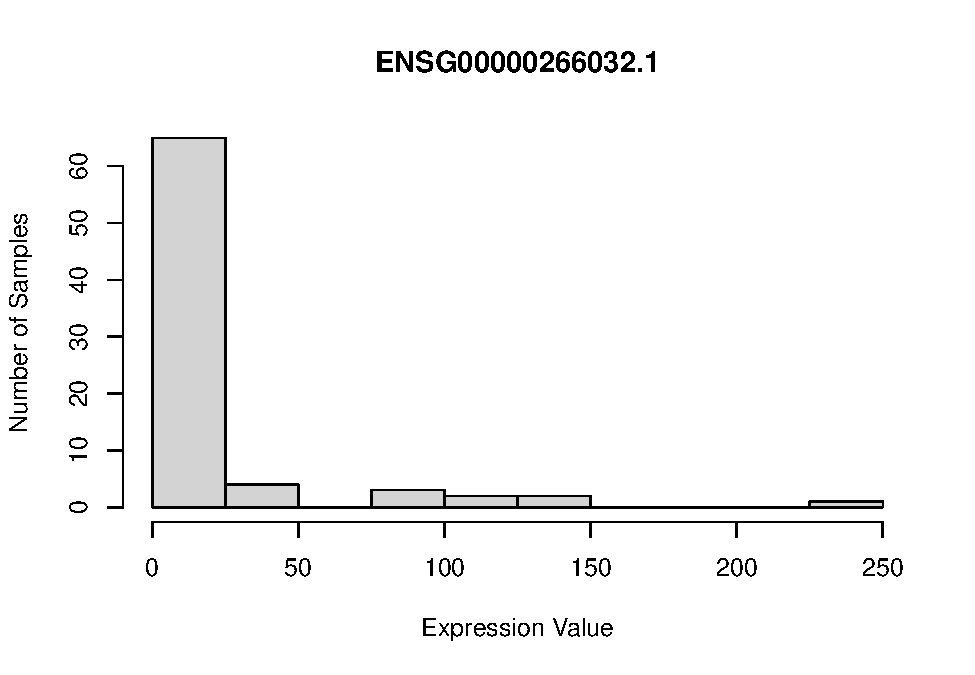
\includegraphics[keepaspectratio]{Assignment_1_Introduction_to_R_files/figure-latex/unnamed-chunk-2-1.pdf}}

\begin{Shaded}
\begin{Highlighting}[]
\DocumentationTok{\#\# Subset this data to contain only their first three samples and first 2000 genes. Write this subset to a file called "eso\_sub.csv". \#\#}

\NormalTok{subset\_data }\OtherTok{\textless{}{-}}\NormalTok{ assignment\_1\_data[}\FunctionTok{c}\NormalTok{(}\DecValTok{1}\SpecialCharTok{:}\DecValTok{2000}\NormalTok{),}\FunctionTok{c}\NormalTok{(}\DecValTok{1}\SpecialCharTok{:}\DecValTok{4}\NormalTok{)] }\CommentTok{\# Subset the data to the first 2000 genes (first 2000 rows) and first three samples (columns 2{-}4, retaining column 1 with the gene labels)}

\FunctionTok{write.csv}\NormalTok{(subset\_data, }\AttributeTok{file =} \StringTok{"eso\_sub.csv"}\NormalTok{) }\CommentTok{\# Write the subsetted data to the csv }
\end{Highlighting}
\end{Shaded}

\begin{enumerate}
\def\labelenumi{\arabic{enumi})}
\setcounter{enumi}{2}
\tightlist
\item
  Write a function call ``my\_first\_function''. The function should
  take the following vector: my\_vector \textless- c(1,2,3,4,5,6,7,8,9).
  Your function should sort the numbers in my\_vector into two
  categories: less than or equal to 5 or greater than 5. Hint: You can
  take a look at for loops and if/else statements to complete this
  question!
\end{enumerate}

\begin{Shaded}
\begin{Highlighting}[]
\NormalTok{my\_first\_function }\OtherTok{\textless{}{-}} \ControlFlowTok{function}\NormalTok{(unsorted\_vector)\{ }\CommentTok{\# Define function name}
\NormalTok{  output\_tbl }\OtherTok{\textless{}{-}} \FunctionTok{data.frame}\NormalTok{(}\AttributeTok{greater\_than\_5 =} \DecValTok{0}\NormalTok{, }\AttributeTok{less\_than\_equal\_5 =} \DecValTok{0}\NormalTok{) }\CommentTok{\# Initialize output table locally (doesn\textquotesingle{}t have to be a dataframe this is just what I chose)}
  \ControlFlowTok{for}\NormalTok{(i }\ControlFlowTok{in} \FunctionTok{seq\_along}\NormalTok{(my\_vector))\{ }\CommentTok{\# Sequence over vector using indices}
    \ControlFlowTok{if}\NormalTok{(my\_vector[i] }\SpecialCharTok{\textgreater{}} \DecValTok{5}\NormalTok{)\{ }\CommentTok{\# Check for the value compared to 5}
\NormalTok{      output\_tbl}\SpecialCharTok{$}\NormalTok{greater\_than\_5[[}\DecValTok{1}\NormalTok{]] }\OtherTok{=}\NormalTok{ output\_tbl}\SpecialCharTok{$}\NormalTok{greater\_than\_5[[}\DecValTok{1}\NormalTok{]] }\SpecialCharTok{+} \DecValTok{1} \CommentTok{\# Increment the value in my data frame if needed}
\NormalTok{    \}}
    \ControlFlowTok{else}\NormalTok{\{ }\CommentTok{\# All other values will be less than or equal to five so no condition (Since our function is designed to take a specific vector with only integers we don\textquotesingle{}t need edge case or error handling)}
\NormalTok{      output\_tbl}\SpecialCharTok{$}\NormalTok{less\_than\_equal\_5[[}\DecValTok{1}\NormalTok{]] }\OtherTok{=}\NormalTok{ output\_tbl}\SpecialCharTok{$}\NormalTok{less\_than\_equal\_5[[}\DecValTok{1}\NormalTok{]] }\SpecialCharTok{+} \DecValTok{1} \CommentTok{\# Increment the value in my data frame if needed}
\NormalTok{    \}}
\NormalTok{  \}}
  \FunctionTok{return}\NormalTok{(output\_tbl) }\CommentTok{\# Return the output }
\NormalTok{\}}

\NormalTok{my\_vector }\OtherTok{\textless{}{-}} \FunctionTok{c}\NormalTok{(}\DecValTok{1}\NormalTok{,}\DecValTok{2}\NormalTok{,}\DecValTok{3}\NormalTok{,}\DecValTok{4}\NormalTok{,}\DecValTok{5}\NormalTok{,}\DecValTok{6}\NormalTok{,}\DecValTok{7}\NormalTok{,}\DecValTok{8}\NormalTok{,}\DecValTok{9}\NormalTok{) }\CommentTok{\# Initialize the vector as requested}

\NormalTok{categorized\_my\_vector }\OtherTok{\textless{}{-}} \FunctionTok{my\_first\_function}\NormalTok{(my\_vector) }\CommentTok{\# Run my function on the initialized vector}

\NormalTok{categorized\_my\_vector }\CommentTok{\# Print out the table}
\end{Highlighting}
\end{Shaded}

\begin{verbatim}
##   greater_than_5 less_than_equal_5
## 1              4                 5
\end{verbatim}

\end{document}
